\documentclass{article}
\usepackage{palatino}
\usepackage[letterpaper,left=0.8in,right=0.8in,top=0.8in,bottom=0.8in]{geometry}
\usepackage{graphicx}
\usepackage{array}
\usepackage{palatino}

\pagestyle{empty}

\begin{document}

\Large

\noindent Name (print): \line(1,0){250} \hspace{0.35in} Userid:
\line(1,0){70}

\vspace{0.25in}

\noindent {\huge Lab 5 AVL Tree worksheet}

\vspace{0.25in}

\noindent {\bf Directions:} Insert the following elements into the
trees shown.  Draw the resulting tree.

\vspace{0.25in}

\noindent\begin{tabular}{lcc}
\bf 1) Insert F & & \bf Tree after insertion: \\
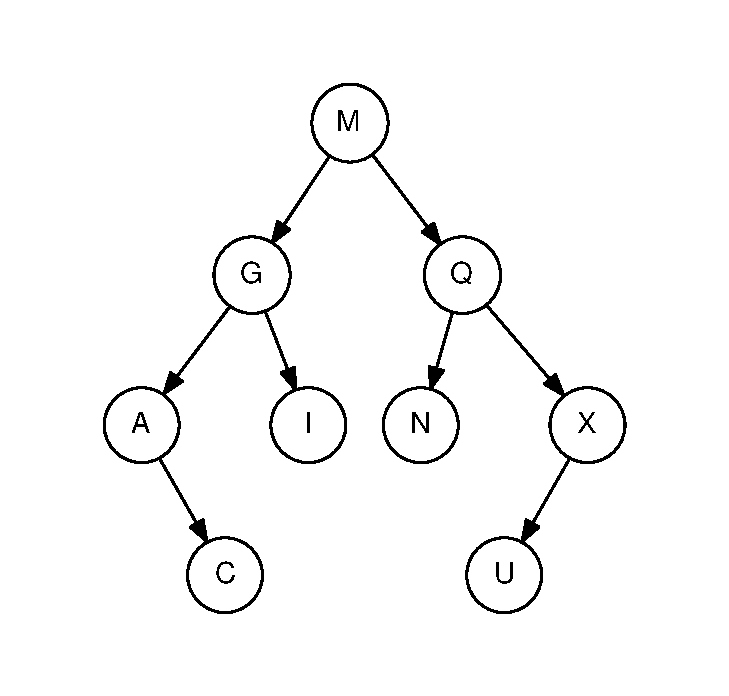
\includegraphics[width=3in]{avl-tree-1} & \hspace{0.5in} & \\
\end{tabular}

\vspace{0.25in}

\noindent\begin{tabular}{lcc}
\bf 2) Insert N & & \bf Tree after insertion: \\
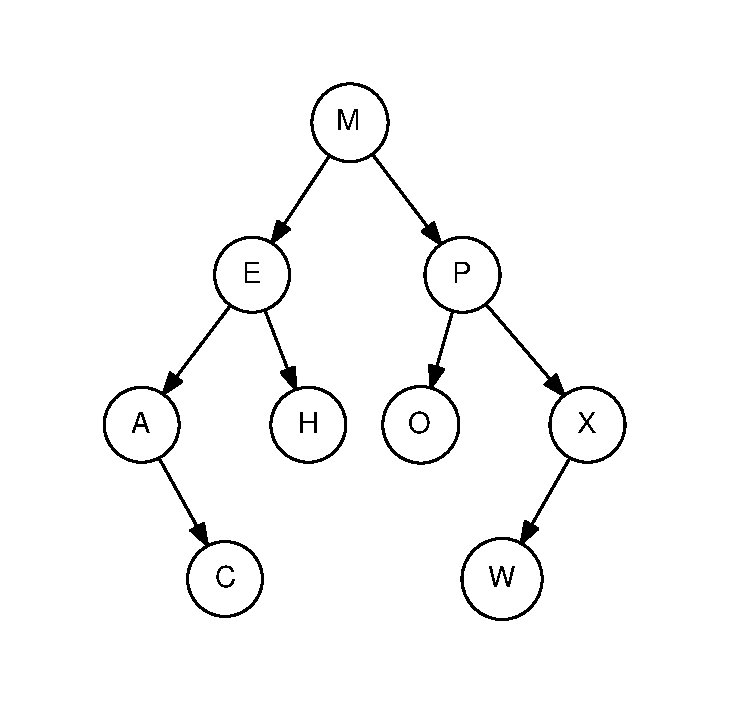
\includegraphics[width=3in]{avl-tree-2} & \hspace{0.5in} & \\
\end{tabular}

\clearpage

\Large

\noindent Name (print): \line(1,0){250} \hspace{0.35in} Userid:
\line(1,0){70}

\vspace{0.25in}

\noindent {\huge Lab 5 AVL Tree worksheet, page 2}
\vspace{0.5in}

\noindent\begin{tabular}{lcc}
\bf 3) Insert B & & \bf Tree after insertion: \\
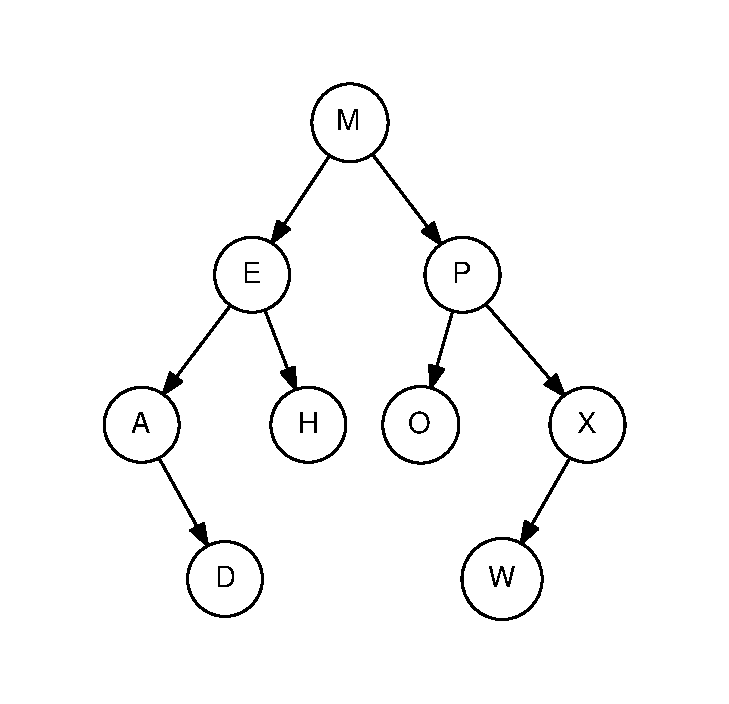
\includegraphics[width=3in]{avl-tree-3} & \hspace{0.5in} & \\
\end{tabular}

\vspace{1.5in}

\noindent\begin{tabular}{lcc}
\bf 4) Insert V & & \bf Tree after insertion: \\
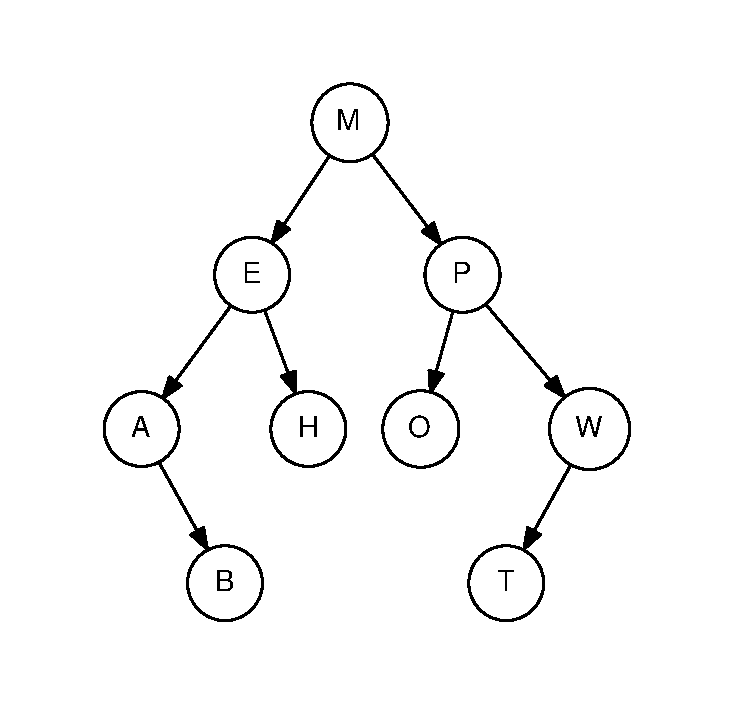
\includegraphics[width=3in]{avl-tree-4} & \hspace{0.5in} & \\
\end{tabular}

\end{document}
